%TC:ignore
\begin{table}[H]
    \caption{Results on ORLIB instances}\label{table:orlib_cost}
    \tiny
    \begin{tabularx}{\textwidth}{XXlXXXXlXXXXlXXXX}
    \firsthline
    \multicolumn{2}{c}{Instance}& \quad & \multicolumn{4}{c}{gon}& \quad & \multicolumn{4}{c}{grasp}& \quad & \multicolumn{4}{c}{pbs}\\
    \cline{1-2} \cline{4-7} \cline{9-12} \cline{14-17}\\
    name & opt && min & $\mu$ & $\sigma$ & \%-gap (opt) && min & $\mu$ & $\sigma$ & \%-gap (opt) && min & $\mu$ & $\sigma$ & \%-gap (opt)\\
    \hline
    pmed1 & 127.00 && 186.00 & 186.00 & 0.00 & 46.00 && 127.00 & 127.34 & 0.68 & 0.00 && 127.00 & 127.00 & 0.00 & 0.00\\
    pmed2 & 98.00 && 131.00 & 131.00 & 0.00 & 34.00 && 102.00 & 106.38 & 2.01 & 9.00 && 98.00 & 98.00 & 0.00 & 0.00\\
    pmed3 & 93.00 && 154.00 & 154.00 & 0.00 & 66.00 && 96.00 & 101.90 & 1.63 & 10.00 && 94.00 & 94.00 & 0.00 & 1.00\\
    pmed4 & 74.00 && 114.00 & 114.00 & 0.00 & 54.00 && 84.00 & 87.10 & 2.51 & 18.00 && 79.00 & 79.00 & 0.00 & 7.00\\
    pmed5 & 48.00 && 71.00 & 71.00 & 0.00 & 48.00 && 59.00 & 63.28 & 1.96 & 32.00 && 50.00 & 52.18 & 0.91 & 9.00\\
    pmed6 & 84.00 && 138.00 & 138.00 & 0.00 & 64.00 && 85.00 & 87.56 & 1.77 & 4.00 && 84.00 & 84.00 & 0.00 & 0.00\\
    pmed7 & 64.00 && 96.00 & 96.00 & 0.00 & 50.00 && 69.00 & 73.48 & 1.53 & 15.00 && 64.00 & 64.00 & 0.00 & 0.00\\
    pmed8 & 55.00 && 81.00 & 81.00 & 0.00 & 47.00 && 67.00 & 69.68 & 1.33 & 27.00 && 58.00 & 58.00 & 0.00 & 5.00\\
    pmed9 & 37.00 && 57.00 & 57.00 & 0.00 & 54.00 && 50.00 & 55.00 & 2.01 & 49.00 && 56.00 & 56.00 & 0.00 & 51.00\\
    pmed10 & 20.00 && 31.00 & 31.00 & 0.00 & 55.00 && 32.00 & 38.08 & 1.74 & 90.00 && 25.00 & 25.82 & 0.89 & 29.00\\
    pmed11 & 59.00 && 73.00 & 73.00 & 0.00 & 24.00 && 59.00 & 61.16 & 1.10 & 4.00 && 59.00 & 59.96 & 0.20 & 2.00\\
    pmed12 & 51.00 && 71.00 & 71.00 & 0.00 & 39.00 && 55.00 & 59.90 & 1.35 & 17.00 && 55.00 & 65.94 & 7.75 & 29.00\\
    pmed13 & 36.00 && 59.00 & 59.00 & 0.00 & 64.00 && 45.00 & 47.28 & 0.78 & 31.00 && 37.00 & 37.00 & 0.00 & 3.00\\
    pmed14 & 26.00 && 41.00 & 41.00 & 0.00 & 58.00 && 40.00 & 44.88 & 1.68 & 73.00 && 33.00 & 34.32 & 1.19 & 32.00\\
    pmed15 & 18.00 && 25.00 & 25.00 & 0.00 & 39.00 && 34.00 & 35.90 & 1.00 & 99.00 && 21.00 & 22.26 & 0.93 & 24.00\\
    pmed16 & 47.00 && 84.00 & 84.00 & 0.00 & 79.00 && 47.00 & 48.10 & 0.46 & 2.00 && 47.00 & 47.00 & 0.00 & 0.00\\
    pmed17 & 39.00 && 56.00 & 56.00 & 0.00 & 44.00 && 42.00 & 43.76 & 0.59 & 12.00 && 39.00 & 39.00 & 0.00 & 0.00\\
    pmed18 & 28.00 && 44.00 & 44.00 & 0.00 & 57.00 && 38.00 & 41.60 & 1.37 & 49.00 && 38.00 & 38.00 & 0.00 & 36.00\\
    pmed19 & 18.00 && 29.00 & 29.00 & 0.00 & 61.00 && 30.00 & 31.42 & 0.87 & 75.00 && 23.00 & 24.96 & 0.28 & 39.00\\
    pmed20 & 13.00 && 18.00 & 18.00 & 0.00 & 38.00 && 28.00 & 30.96 & 1.47 & 138.00 && 17.00 & 18.58 & 0.92 & 43.00\\
    pmed21 & 40.00 && 53.00 & 53.00 & 0.00 & 32.00 && 40.00 & 42.08 & 0.66 & 5.00 && 40.00 & 40.00 & 0.00 & 0.00\\
    pmed22 & 38.00 && 56.00 & 56.00 & 0.00 & 47.00 && 43.00 & 44.04 & 0.28 & 16.00 && 39.00 & 39.88 & 0.68 & 5.00\\
    pmed23 & 22.00 && 34.00 & 34.00 & 0.00 & 55.00 && 32.00 & 34.44 & 1.17 & 57.00 && 26.00 & 26.92 & 0.27 & 22.00\\
    pmed24 & 15.00 && 23.00 & 23.00 & 0.00 & 53.00 && 26.00 & 28.34 & 1.05 & 89.00 && 19.00 & 20.88 & 0.47 & 39.00\\
    pmed25 & 11.00 && 16.00 & 16.00 & 0.00 & 45.00 && 23.00 & 28.56 & 2.41 & 160.00 && 15.00 & 15.04 & 0.20 & 37.00\\
    pmed26 & 38.00 && 50.00 & 50.00 & 0.00 & 32.00 && 39.00 & 40.00 & 0.66 & 5.00 && 38.00 & 38.04 & 0.28 & 0.00\\
    pmed27 & 32.00 && 43.00 & 43.00 & 0.00 & 34.00 && 35.00 & 35.78 & 0.54 & 12.00 && 33.00 & 33.00 & 0.00 & 3.00\\
    pmed28 & 18.00 && 28.00 & 28.00 & 0.00 & 56.00 && 27.00 & 28.84 & 0.99 & 60.00 && 26.00 & 26.00 & 0.00 & 44.00\\
    pmed29 & 13.00 && 20.00 & 20.00 & 0.00 & 54.00 && 24.00 & 27.98 & 2.29 & 115.00 && 18.00 & 18.02 & 0.14 & 39.00\\
    pmed30 & 9.00 && 14.00 & 14.00 & 0.00 & 56.00 && 24.00 & 26.22 & 1.79 & 191.00 && 12.00 & 12.92 & 0.34 & 44.00\\
    pmed31 & 30.00 && 42.00 & 42.00 & 0.00 & 40.00 && 31.00 & 32.18 & 0.62 & 7.00 && 30.00 & 30.02 & 0.14 & 0.00\\
    pmed32 & 29.00 && 45.00 & 45.00 & 0.00 & 55.00 && 31.00 & 32.98 & 0.71 & 14.00 && 31.00 & 60.80 & 17.96 & 110.00\\
    pmed33 & 15.00 && 25.00 & 25.00 & 0.00 & 67.00 && 24.00 & 25.90 & 1.32 & 73.00 && 19.00 & 19.00 & 0.00 & 27.00\\
    pmed34 & 11.00 && 17.00 & 17.00 & 0.00 & 55.00 && 23.00 & 26.38 & 1.73 & 140.00 && 15.00 & 15.32 & 0.47 & 39.00\\
    pmed35 & 30.00 && 38.00 & 38.00 & 0.00 & 27.00 && 31.00 & 32.68 & 0.55 & 9.00 && 30.00 & 30.42 & 0.60 & 1.00\\
    pmed36 & 27.00 && 41.00 & 41.00 & 0.00 & 52.00 && 30.00 & 31.70 & 0.78 & 17.00 && 29.00 & 40.76 & 3.72 & 51.00\\
    pmed37 & 15.00 && 25.00 & 25.00 & 0.00 & 67.00 && 24.00 & 26.88 & 1.32 & 79.00 && 19.00 & 19.00 & 0.00 & 27.00\\
    pmed38 & 29.00 && 39.00 & 39.00 & 0.00 & 34.00 && 29.00 & 32.08 & 1.15 & 11.00 && 40.00 & 40.00 & 0.00 & 38.00\\
    pmed39 & 23.00 && 35.00 & 35.00 & 0.00 & 52.00 && 25.00 & 26.54 & 0.70 & 15.00 && 74.00 & 74.00 & 0.00 & 222.00\\
    pmed40 & 13.00 && 21.00 & 21.00 & 0.00 & 62.00 && 22.00 & 24.04 & 1.17 & 85.00 && 18.00 & 18.00 & 0.00 & 38.00\\
    \hline
    \multicolumn{2}{l}{Average} &&&&& 49.87 &&&&& 47.83 &&&&& 27.38\\
    \hline
    \multicolumn{4}{r}{Quade test on mean costs} & \multicolumn{3}{l}{p-value=\num{7.25e-9}} & \multicolumn{10}{c}{}\\
    \lasthline
    \end{tabularx}
    \normalsize
\end{table}
%TC:endignore

\paragraph{Analysis of solution cost}~\\
The Quade omnibus test (\Cref{method:quade_test})  returned a p-value of \num{7.25e-9} (\cref{table:orlib_cost}). Since it is statistically significant, we perform a post-hoc Quade test (\Cref{method:post_hoc_quade}), the results are shown in \cref{table:post_hoc_orlib}.

%TC:ignore
\begin{table}[H]
    \centering
    \caption{P-values from post-hoc Quade test on ORLIB $\mu$ costs}\label{table:post_hoc_orlib}
    \begin{tabularx}{0.75\textwidth}{|X|XX|}
        \hline
        \textbf{Algorithm} & \emph{Gon} & GRASP Plateau Surfer\\
        \hline
        GRASP Plateau Surfer & \num{4.14e-3} & N/A\\
        PBS & \num{3.46e-9} & \num{3.30e-4}\\
        \lasthline
    \end{tabularx}
\end{table}
%TC:endignore

All three pairwise Quade tests returned a p-value below 0.05, we evaluate the three algorithms using \Cref{method:counting_results} and report it in \cref{fig:compare_three_alg}. PBS achieved a lower cost than the \emph{Gon} algorithm in 36/40 and \acrshort{grasp_ps} in 34/40 ORLIB problems. Similarly \acrshort{grasp_ps} performed better than the \emph{Gon} in 25/40 problem instances. 

%TC:ignore
\begin{figure}[H]
    \begin{minipage}{0.57\textwidth}
        \centering
        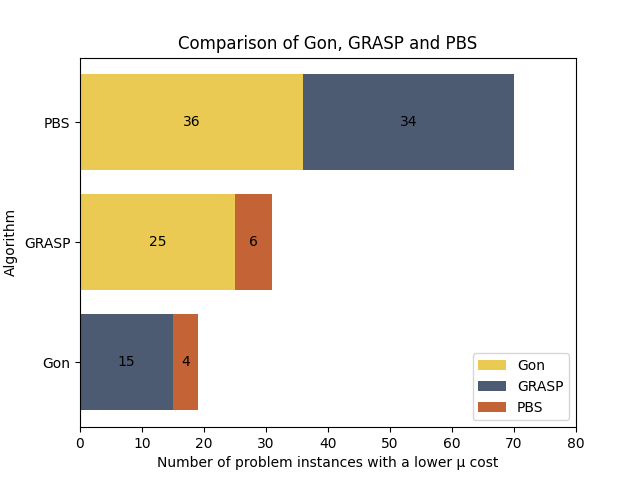
\includegraphics[width=\textwidth]{images/compare_three_alg.png}
        \caption{Number of problem instances where an\newline algorithm performed better than another (higher\newline is better)}
        \label{fig:compare_three_alg}
    \end{minipage}
    \begin{minipage}{0.43\textwidth}
        \centering
        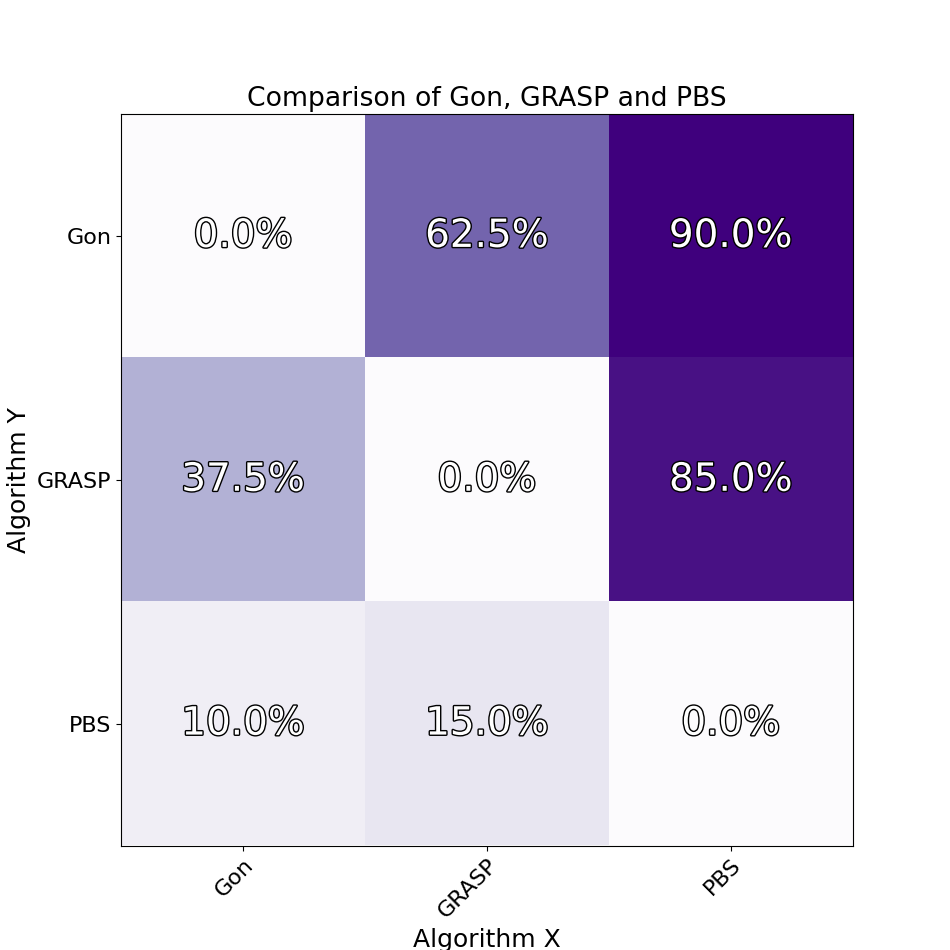
\includegraphics[width=\textwidth]{images/k_center_conf_matrix.png}
        \caption{\% of ORLIB instances where algorithm X performed better than algorithm Y (higher is better)}
        \label{fig:compare_three_alg_conf_matrix}
    \end{minipage}
\end{figure}
%TC:endignore

We account for variance using \Cref{method:counting_results_variance} with $\Delta =2$ which accounts for 95\% of the data under a normal distribution. Notably, PBS achieves a lower cost than \acrshort{grasp_ps} for 34/40 instances and 31/40 for the \emph{Gon} algorithm. %show full results%

The average \%-gap above optimal cost was $\mu$ was 49.87\%, 47.83\% and 27.38\% for \emph{Gon}, Grasp Plateau Surfer and PBS respectively. While we observed strong results for PBS, we could not reproduce results by \textcite{pullan_memetic_2008} which showed the optimal optimal cost could be reached on all ORLIB problems. A possible reason could be PBS's strategy to maintain population diversity, something that was mentioned but not detailed in their paper. We contacted the author via email for clarification but we did not receive a reply.

Overall, accounting for variance, the best algorithm for the $k$-center is \acrshort{pbs} followed by \acrshort{grasp_ps} and the worst performing is the \emph{Gon} algorithm.